\documentclass[11pt]{article}
\usepackage{graphicx}
\usepackage{hyperref}
\usepackage{appendix}
\usepackage{amsmath}
\usepackage{amsthm}
\usepackage{amssymb}
\usepackage{float}
\usepackage{commath}
\usepackage{booktabs}
\renewcommand{\arraystretch}{1.2}
\usepackage{siunitx}
\sisetup{detect-all}
\usepackage{listings}
\usepackage{color} %red, green, blue, yellow, cyan, magenta, black, white
\definecolor{mygreen}{RGB}{28,172,0} % color values Red, Green, Blue
\definecolor{mylilas}{RGB}{170,55,241}
\usepackage[a4paper,margin=20mm]{geometry}
\numberwithin{equation}{section}
\setlength{\parskip}{\baselineskip}
\setlength{\parindent}{0pt}
\hypersetup{
    colorlinks=true,
    linkcolor=black,
    filecolor=black,      
    urlcolor=black,
    citecolor=black
}
\urlstyle{same}
\begin{document}
\title{\textbf{UCL Mechanical Engineering 2020/2021}\\MECH0010 Final Assessment}
\author{NCWT3}
\maketitle
\tableofcontents
\listoffigures
\section{Question 1}
\subsection{a}
\begin{figure}[H]
   \centering
   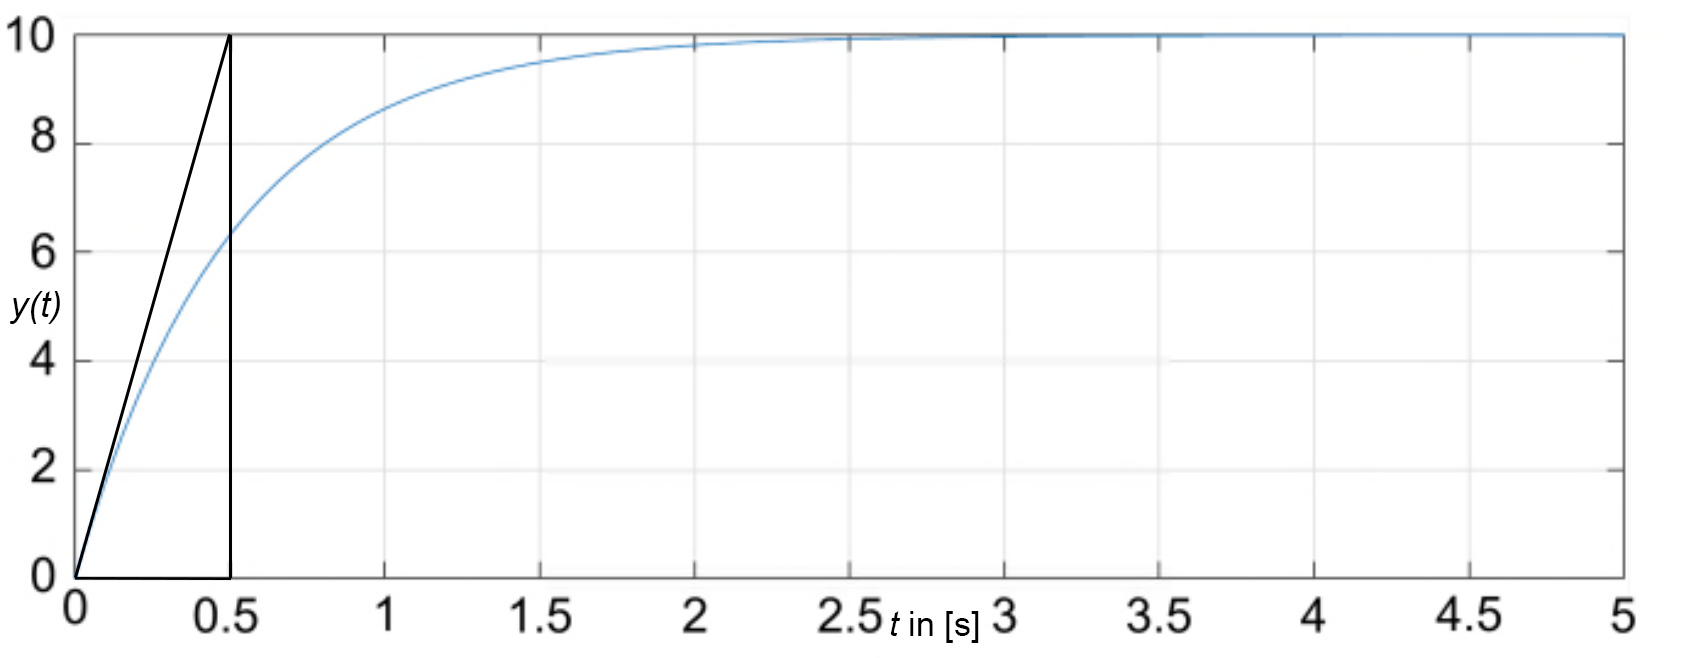
\includegraphics[width = 0.9 \textwidth]{./img/q1i1.png}
   \caption{Diagram to show step response of a first-order system.} 
   \label{fig:q1i1}
\end{figure}
Let us look at \ref{eq:q1i1}
\begin{equation}
    \frac{\dif y(t)}{\dif t} = ay(t) + b u(t)\label{eq:q1i1}
\end{equation}
Transforming to Laplace domain:
\begin{align}
    sY(s) - y(0) &= aY(s) + bU(s)
\end{align}
$y(0) = 0$:
\begin{align}
    Y(s)\left(s-a\right) &= bU(s)\\
    \frac{Y(s)}{U(s)} = \frac{b}{s-a}
\end{align}
For step input $U(s) = \frac{1}{s}$:
\begin{gather}
    Y(s) = \frac{b}{s(s-a)} = \frac{k_1}{s}+ \frac{k_2}{s-a}
\end{gather}
Solving partial fraction:
\begin{gather}
    k_1(s-a) + k_2 s = b\\
    s = 0 \rightarrow -ak_1 = b\\
    k_1 = -\frac{b}{a}\\
    s = a \rightarrow ak_2 = b\\
    k_2 = \frac{b}{a}\\
    Y(s) = \frac{b}{a(s-a)} - \frac{b}{as}\\
    Y(s) = \frac{b}{a}\left(\frac{1}{s-a}-\frac{1}{s}\right)
\end{gather}
Returning to time domain (using tables):
\begin{gather}
    y(t) = \frac{b}{a} \left(e^{at}-1\right) \label{eq:q1i2}\\
    \frac{\dif y(t)}{\dif t} = be^{at}\\
    \left. \frac{\dif y(t)}{\dif t} \right|_{t = 0} = b
\end{gather}
From Figure \ref{fig:q1i1}, we can see that the gradient at 0 is:
\begin{equation}
    b = \frac{10}{0.5} = 20
\end{equation}
Response settles at $y(t) = 10$, therefore:
\begin{align}
    e^{at} &= 0\\
    \therefore 10 &= \frac{20}{a}\left(-1\right)\\
    a &= -2
\end{align}
Hence:
\begin{align}
    y(t) = -10 \left(e^{-2t}-1\right)\\
    \frac{\dif y(t)}{\dif t} = -2y(t) + 10u(t)
\end{align}
\subsection{b}
\subsubsection{i}
\begin{align}
    \frac{\dif \omega(t)}{\dif t} &= -a\omega(t) + kv(t)\\
    s \Omega(s) - \omega(0) &= -a \Omega(s) + kV(s)\\
    s\Omega(s) +a\Omega (s) &= kV(s)\\
    \Omega(s)\left(s+a\right) &= kV(s)\\
    \frac{\Omega (s)}{V(s)} &= \frac{k}{s+a}\\
    \frac{\Omega (s)}{V(s)} &= \frac{\frac{k}{a}}{\frac{s}{a}+1} = \frac{\gamma}{\tau s + 1}
\end{align}
Where $\gamma$ is the gain and $\tau$ is the time constant.
\section{Question 2}
To measure the temperature of the gas flow , we can utilise a simple thermistor. A thermistor changes resistance based on the local environmental temperature. The Steinhart-Hart equation provides a precise measurement of temperature from a thermistor (\ref{eq:q2i2}). 
\begin{equation}
    \frac{1}{T} = A + B \ln R + C \left(\ln R\right)^3 \label{eq:q2i2}
\end{equation}
Thermistors are small and can be positioned in the flow easily. An important design consideration is to make sure that it is placed near the centre of flow for an accurate reading, due to boundary layer effects. 

To measure gas flow, we will be utilising a voltage based measurement from a hot wire anemometer, specifically a constant temperature anemometer. They are small, thin wires suspended in the flow, heated by a current. A circuit diagram is shown in Figure \ref{fig:q2i1}
\begin{figure}[H]
    \centering
    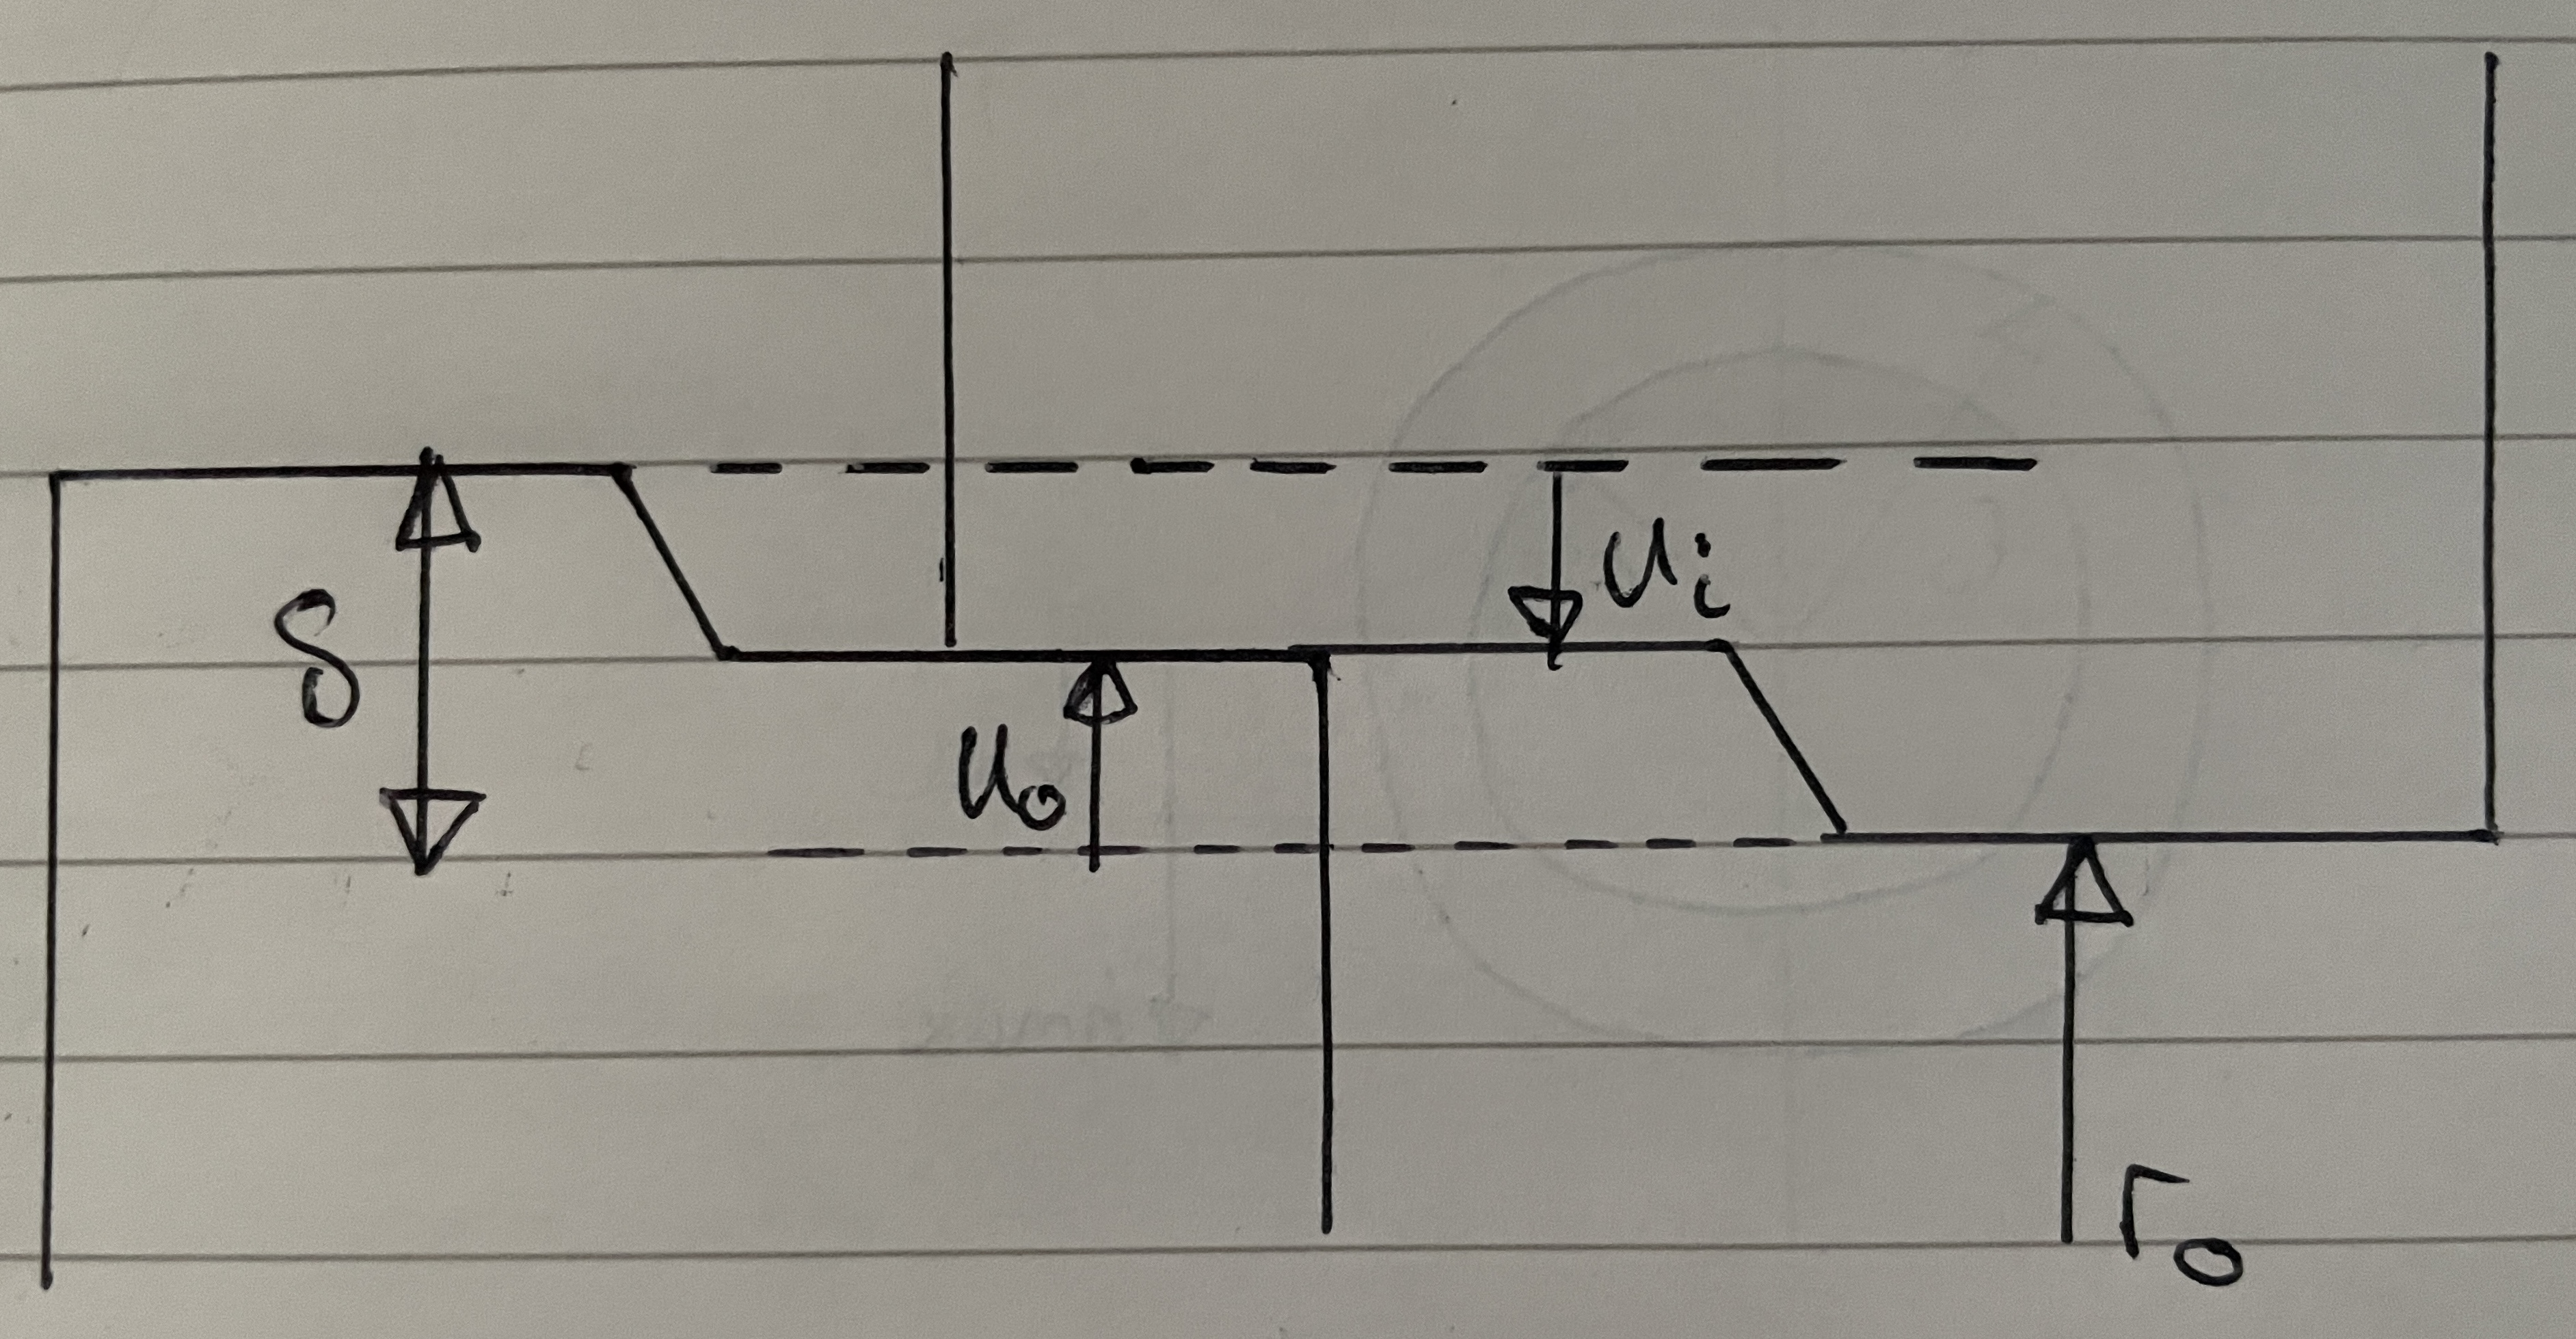
\includegraphics[height = 5cm]{./img/q2i1.jpg}
    \caption{Diagram to show basic circuit for a hot wire anemometer working on constant temperature mode.} 
    \label{fig:q2i1}
 \end{figure}
We know that the resistance of a wire is proportional to its temperature and if we can maintain the temperature at a certain value, then we will be able to maintain its resistance. Initially our bridge is balanced and as fluid flows past our wire, there is heat transfer at a constant rate. As the velocity of the fluid changes, the rate of thermal heat transfer also changes. In the case that flow rate increases, the increased heat transfer causes the temperature of the wire to decrease, decreasing its resistance. This causes the bridge to become unbalanced. From Figure \ref{fig:q2i1}, an $e^+$ signal is sent to the op-amp. After amplification, the bridge voltage is increased and current flow through the wire is increased. An increase in current, leads to an increase in temperature and resistance, balancing the bridge \cite{b1}. 

Use of a hot wire anemometer is justified as they are small sensors (millimetre scale) and can be used in high temperature situations. The TSI model 1222 can be used in fluids up to \SI{300}{\celsius} \cite{b3}. They have high frequency response but are fragile, expensive and require clean gas flows to prevent damage \cite{b3}. As stated previously, it should be placed close to the centre of flow. \ref{eq:q2i1} is an equation for the fluid velocity as a function of current $I$, calibration resistance and temperature $R_i$, $T_i$, wire and fluid temperatures $T_w$, $T_f$ and projected surface area of wire $A_w$ \cite{b2}.
\begin{align}
    v_f = \left[\frac{I^2 R_{i}\left[1 + \alpha \left(T_w - T_i\right)\right]}{BA_w \left(T_w - T_f\right)}-\frac{A}{B}\right]^{\frac{1}{c}} \label{eq:q2i1}
\end{align}
Strain gauges can be used to measure changes in the pipes geometry. A simple Wheatstone bridge arrangement of strain gauges, will allow us to measure the vibrations in the pipe. As the pipe is small and we would like to make accurate measurements of vibration, a semiconductor strain gauge may be used. 
\begin{figure}[H]
    \centering
    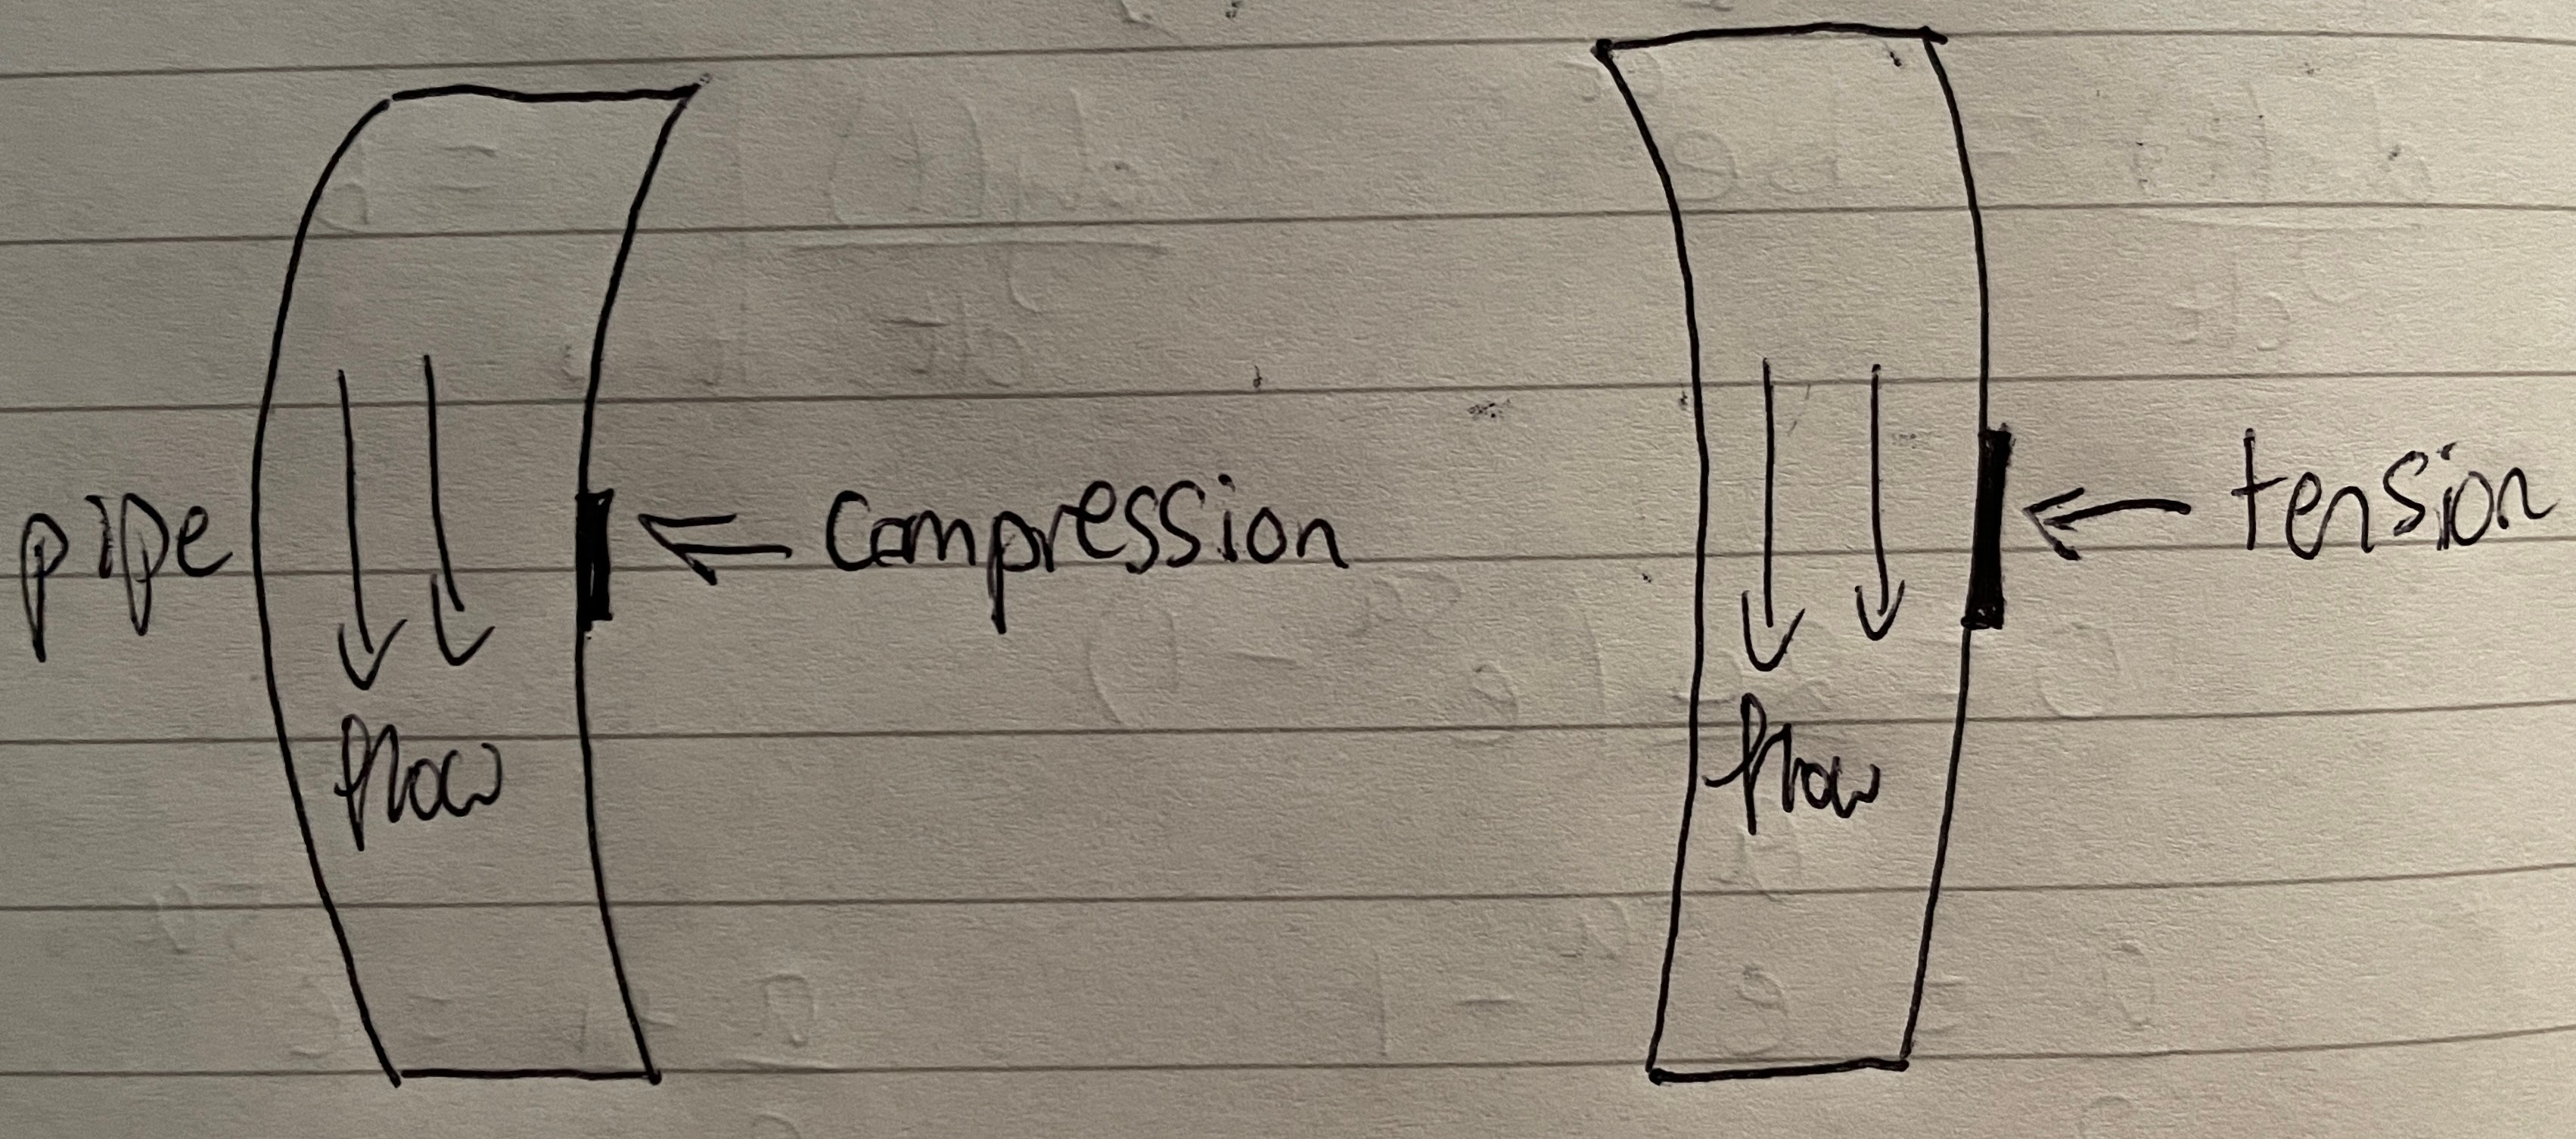
\includegraphics[height = 4cm]{./img/q2i3.jpg}
    \caption{Diagram to show how vibrations in the pipe change the shape of a strain gauge fixed to the outer surface.} 
    \label{fig:q2i3}
\end{figure}
\begin{figure}[H]
    \centering
    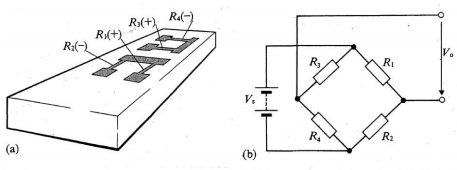
\includegraphics[height = 4cm]{./img/q2i2.png}
    \caption{Diagram to show basic circuit for a semiconductor strain gauge, with temperature compensation.} 
    \label{fig:q2i2}
\end{figure}
The bridge output is given as:
\begin{align}
    V_0 = \frac{V_s x }{2} \left(1 + \nu\right)
\end{align}
\begin{thebibliography}{00}
    \bibitem{b1} Howard Hodson, University of Cambridge, Department of Engineering, Whittle Laboratory "Constant Temperature Anemometers", \url{http://www-g.eng.cam.ac.uk/whittle/current-research/hph/cta-circuit/cta-circuit.html} Accessed 10/05/21 23:05 
    \bibitem{b3} TSI, "TSI Thermal Anemometry Probes", \url{https://www.tsi.com/getmedia/2e3fafd5-8037-40a9-aa38-4fa05a1d3ef3/Hotwire_Catalog_2980465?ext=.pdf} Accessed 11/05/21 00:43
    \bibitem{b2} eFunda Inc, "Hot wire theory", \url{https://www.efunda.com/designstandards/sensors/hot_wires/hot_wires_intro.cfm} Accessed 11/05/21 00:09
\end{thebibliography}
\end{document}